\subsection{Experimental Principle of Targeted Memory Reactivation}

Targeted Memory Reactivation (TMR) is an experimental procedure for biasing
post-encoding memory processing through sensory cues associated with prior
learning. During wakefulness, a sound, odor, or other stimulus is paired with
specific learned information. Re-presentation of that cue during subsequent
sleep can selectively influence later retention of the associated material
\citep{rasch2007odor,rudoy2009strengthening,oudiette2013upgrading}. TMR
therefore does not introduce information into memory during sleep; it acts on
representations established before sleep by providing an external signal linked
to the earlier learning episode.

The mechanistic interpretation of this effect requires caution. A selective
behavioral benefit following cueing is evidence that the cue altered
post-encoding memory processing, but it does not by itself demonstrate the
precise neural content or pathway of reactivation. Neuroimaging and
electrophysiological studies provide additional evidence that sleep-time cues
can evoke learning-related activity and content-specific neural patterns
\citep{rasch2007odor,cairney2018spindle,wang2019signals}. The most defensible
interpretation is therefore that appropriately associated cues can bias
endogenous memory reactivation during sleep, while the exact neural sequence
linking cue perception to later behavioral improvement remains incompletely
resolved.

This distinction separates TMR from nonspecific sensory stimulation. Its
experimental logic depends on three linked conditions: the existence of a
pre-sleep cue--memory association, presentation of the cue under an appropriate
physiological condition, and a subsequent difference in memory attributable to
the cueing manipulation. These conditions form the basis for evaluating both
TMR efficacy and its later translation into an automated intervention.


\subsection{Encoding and Cue--Memory Association}

The effectiveness of TMR is constrained by what has been learned before sleep.
A cue can only influence a memory insofar as it has acquired a meaningful
relationship with the target representation during encoding. Evidence from
object--location and associative-learning paradigms indicates that prior memory
strength and the directness of the cue--memory association can influence the
magnitude of subsequent TMR effects
\citep{creery2015priorlearning,cairney2016benefits}.

This relationship is more nuanced than a simple requirement for maximally strong
encoding. Creery et al.\ found that near-perfectly learned spatial memories did
not show the same TMR benefit as less completely learned memories, while Cairney
et al.\ reported stronger effects for memories recalled with relatively low
pre-sleep accuracy and found evidence that direct cue--memory associations were
important for successful reactivation
\citep{creery2015priorlearning,cairney2016benefits}. TMR should therefore not
be described as rescuing memories that were never encoded, but neither should
weak pre-sleep performance automatically be treated as a failure condition.

Cue specificity also affects interpretation. Item-specific auditory cues can
permit selective comparison between cued and uncued memories, as demonstrated
by Rudoy et al., whereas contextual cues such as odors can reactivate a broader
learning context \citep{rasch2007odor,rudoy2009strengthening}. Behavioral
selectivity should not be equated with complete neural isolation: a cue may
reactivate features of the target memory together with contextual or associated
representations. For translational purposes, the critical requirement is
therefore not maximal cue uniqueness in the abstract, but a reproducible
association between the cue and the memory process the intervention is intended
to influence.


\subsection{Physiological Conditions for State-Dependent Cueing}

TMR efficacy depends not only on what is cued, but also on the physiological
state in which cueing occurs. The meta-analysis by Hu et al.\ found significant
positive effects for cueing during NREM stage~2
(\(g=0.32\), 95\% CI \(0.04\)--\(0.60\)) and slow-wave sleep
(\(g=0.27\), 95\% CI \(0.20\)--\(0.35\)), whereas pooled effects for REM sleep
and wakefulness were not significant
\citep{hu2020promoting}. These results support NREM sleep as the best-established
cueing context in the literature synthesized by that analysis, but they do not
establish that a single sleep stage is universally optimal for every memory
domain or experimental objective.

The physiological context described in Section~3 provides a plausible basis for
this state dependence. During NREM sleep, slow oscillations, sleep spindles, and
hippocampal activity associated with memory reprocessing exhibit structured
temporal relationships
\citep{rasch2013sleep,klinzing2019mechanisms,staresina2015nesting}. TMR cues
enter this ongoing physiological environment rather than initiating
consolidation independently. Accordingly, cue timing should be understood as an
interaction with endogenous sleep dynamics rather than as delivery of a stimulus
to a uniformly receptive sleeping brain.

Evidence also indicates that finer temporal structure within NREM can influence
cue efficacy. Cue-induced spindle activity has been associated with successful
memory processing, and manipulation of cue timing relative to spindle dynamics
has demonstrated that some NREM intervals are more favorable than others
\citep{cairney2018spindle,antony2018spindle}. More direct closed-loop evidence
has subsequently tested TMR relative to ongoing slow-oscillation phase.
Shimizu et al.\ implemented an EEG-based closed-loop system that delivered
memory-associated sounds around detected slow-oscillation down-to-up
transitions and reported improved spatial-navigation performance relative to a
non-stimulated control condition \citep{shimizu2018closedloop}. The study
demonstrated the feasibility and behavioral relevance of phase-sensitive
closed-loop TMR, although it did not establish superiority over an otherwise
equivalent open-loop TMR protocol.

Ngo and Staresina later directly compared memory cues delivered during
slow-oscillation UP and DOWN states and found reduced overnight forgetting for
memories cued during UP states relative to DOWN states
\citep{ngo2022shaping}. More recently, Nicolas et al.\ extended this approach
to motor memory and likewise found phase-dependent behavioral and
electrophysiological effects, with greater overnight performance improvement
for UP- than DOWN-reactivated motor sequences
\citep{nicolas2025phase}. Importantly, the UP-reactivated condition in that
study did not significantly outperform the non-reactivated condition,
illustrating that evidence for phase dependence does not yet establish a
general incremental advantage of phase-locked TMR over simpler cueing
strategies.

These findings provide direct empirical support for event- and phase-aware
closed-loop TMR rather than merely a mechanistic rationale for it. The evidence
base is nevertheless narrower than that supporting TMR delivered within broader
NREM conditions, and phase-specific control introduces additional requirements
for causal event detection, phase estimation, synchronization, and cue timing.
Stage-aware and phase-aware control should therefore remain distinct levels of
intervention complexity.

These findings provide the rationale for state-dependent closed-loop control in
an autonomous implementation. TMR itself does not require an automated
closed-loop system; many foundational studies relied on experimenter-supervised
sleep monitoring. For real-world automation, however, physiological information
must replace continuous researcher judgment. Such a system must determine when
cueing is permitted, when it should be withheld, and when evidence of disturbance
should interrupt further stimulation. The quantitative thresholds and algorithms
needed to implement these functions remain engineering and validation questions
rather than established neuroscientific constants.


\begin{figure*}[t]
    \centering
    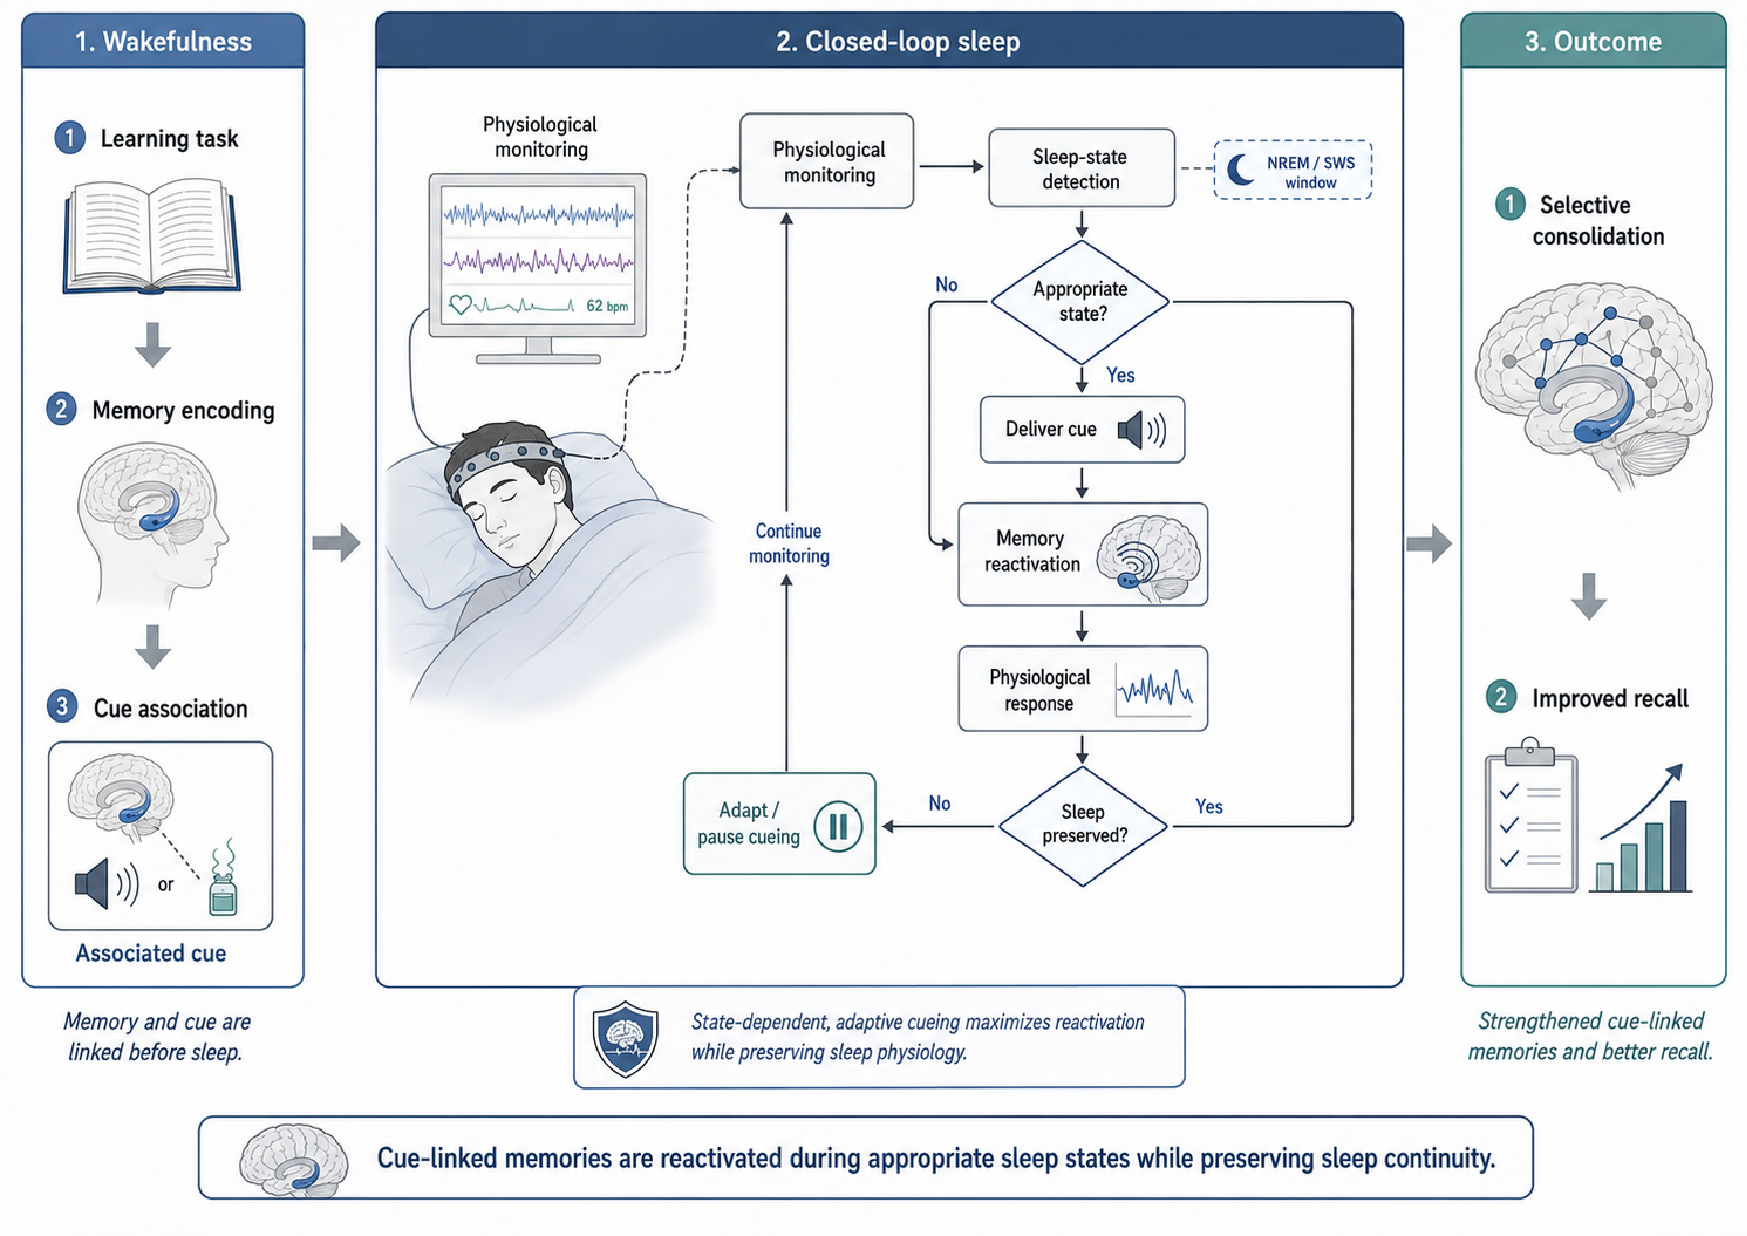
\includegraphics[
        width=\textwidth,
        keepaspectratio
    ]{figures/fig5_TMR_closed_loop.pdf}

    \caption{
    Conceptual workflow for state-dependent closed-loop Targeted Memory
    Reactivation. Sensory cues are first associated with selected information
    during wakeful learning. During subsequent sleep, ongoing physiological
    measurements are used to determine whether the current state is eligible
    for cue presentation. Following stimulation, physiological information can
    be used to evaluate disturbance and determine whether cueing should continue,
    be delayed, or be suspended. The workflow is an original conceptual
    synthesis of experimental and automated TMR paradigms; cue delivery does not
    guarantee memory enhancement, and behavioral efficacy remains an empirical
    outcome
    \citep{oudiette2013upgrading,whitmore2022improving,salfi2025promoting}.
    }
    \label{fig:tmr_closed_loop_process}
\end{figure*}


\subsection{Experimental Evidence for TMR Efficacy and Mechanism}

Early controlled experiments established the fundamental causal effect of
sleep-time cue presentation on later memory performance. Rasch et al.\
re-presented an odor that had been present during learning and found improved
retention of a hippocampus-dependent spatial task when the odor was presented
during slow-wave sleep. The same manipulation was ineffective when the odor had
not been associated with learning and did not produce the corresponding benefit
during wakefulness or REM sleep
\citep{rasch2007odor}. The experiment therefore demonstrated that the behavioral
effect depended jointly on prior association and physiological state rather than
on sensory stimulation alone.

Rudoy et al.\ subsequently demonstrated item-level selectivity using an
object--location task. Individual objects were paired with characteristic sounds
during learning, and only a subset of those sounds was replayed during sleep.
Post-sleep location memory was more accurate for cued than uncued objects
\citep{rudoy2009strengthening}. Because cued and uncued items were learned by
the same individuals and experienced the same sleep period, this within-subject
design provided strong evidence that targeted sensory reminders can alter the
retention of selected memories.

The broader magnitude of the effect was quantified by Hu et al.\ in a multilevel
meta-analysis of 91 experiments, 212 effect sizes, and 2,004 participants.
Across sleep-based TMR experiments, the pooled effect was
Hedges' \(g=0.29\) (95\% CI \(0.21\)--\(0.38\))
\citep{hu2020promoting}. This represents a modest standardized benefit, not a
29\% improvement in memory performance and not an expected effect for every
participant or protocol.

The same meta-analysis also places an important boundary around that estimate.
Effect sizes were substantially heterogeneous
(\(I^2=71\%\)), indicating large variation beyond sampling error. Hu et al.\
also detected funnel-plot asymmetry consistent with possible publication bias;
under one trim-and-fill correction, the estimated overall effect decreased to
\(g=0.18\) (95\% CI \(0.06\)--\(0.30\)) while remaining significantly above
zero \citep{hu2020promoting}. The central quantitative conclusion is therefore
not that TMR produces a fixed effect of \(g=0.29\), but that the literature
supports a small positive average effect whose magnitude is strongly
condition-dependent.

Neurophysiological findings provide convergent but not definitive evidence about
the mechanism underlying this behavioral effect. Cairney et al.\ found that
memory cues increased fast-spindle activity relative to control stimuli and
that memory-category information could be decoded during this spindle response;
the fidelity of decoding predicted later TMR benefit
\citep{cairney2018spindle}. Wang et al.\ likewise identified
content-related EEG activity following sleep-time cues, with stronger
learning-related signals associated with subsequent memory and post-cue spindle
activity \citep{wang2019signals}. Antony et al.\ further showed that
experimentally manipulating cue timing relative to ongoing spindle dynamics
changed later memory performance \citep{antony2018spindle}.

These studies strengthen the interpretation that TMR can engage
memory-specific processing embedded within NREM electrophysiology. They do not,
however, justify treating any single EEG response as a validated surrogate for
successful memory enhancement. Spindle activity and decodable neural patterns
are mechanistically informative, but their relationship to behavioral benefit
remains variable and in several studies correlational. Behavioral outcome
therefore remains necessary when evaluating TMR efficacy.


\subsection{From Laboratory Demonstration to Home-Based Feasibility}

Moving TMR beyond supervised laboratory environments introduces a different
evidentiary question: whether the intervention can preserve its physiological
and behavioral properties when monitoring and cue delivery are automated.
Early unsupervised work demonstrated the difficulty of this transition.
G{\"o}ldi and Rasch applied vocabulary cueing across three nights at home without
online sleep-state control and found no uniform benefit across the full sample;
outcomes depended strongly on reported sleep disturbance and habituation
\citep{goldi2019home}. This result is important because it shows that removing
physiological supervision does not automatically preserve laboratory efficacy.

Whitmore et al.\ subsequently developed SleepStim, which combined smartwatch
movement and heart-rate measurements with a smartphone-based auditory cueing
system. In the first experiment (\(n=61\)), the overall TMR effect was not
significant, although memory outcome varied systematically with sound intensity.
After restricting stimulus intensity in a second experiment (\(n=24\)), cued
spatial memories showed a significant advantage
\citep{whitmore2022improving}. The study provides evidence that automated
peripheral-sensor-guided TMR can operate at home while simultaneously
demonstrating that intervention parameters and sleep disturbance materially
affect the result.

More direct electrophysiological control was demonstrated by Salfi et al.\ using
a Dreem~2 wearable EEG system in 24 adults sleeping at home. Participants
learned translations for 40 pseudowords, half of which were subsequently
re-presented following real-time detection of slow waves. Cued items improved
by 8.6\% from evening test to morning retest, whereas the corresponding change
for uncued items was not significant; morning recall was also higher for cued
than uncued material. Successful recall was associated with greater
post-stimulus spindle-range activity
\citep{salfi2025promoting}.

Taken together, these studies provide proof-of-concept evidence for automated
home TMR across both peripheral and EEG-based sensing approaches
\citep{goldi2019home,whitmore2022improving,salfi2025promoting}. They do not
establish population-level effectiveness, long-term reliability, or equivalence
between sensing modalities. The evidence instead demonstrates a progression
from unsupervised cue playback to physiological state-dependent automation,
while showing that sensing quality, stimulation control, and preservation of
sleep remain central determinants of translational success.


\subsection{Boundary Conditions and Evidence-Derived Implications}

TMR should therefore be interpreted as a condition-dependent intervention rather
than a deterministic memory-enhancement mechanism. Its pooled behavioral effect
is positive but modest, and substantial between-study heterogeneity indicates
that protocol, memory type, sleep state, and participant-level factors materially
influence outcome \citep{hu2020promoting}. Prior memory strength and the
structure of cue--memory associations provide additional sources of variability
\citep{creery2015priorlearning,cairney2016benefits}.

Individual predictability remains particularly limited. Differences in sleep
architecture, sensory threshold, initial learning, cue responsiveness, and
oscillatory physiology may contribute to variation between participants and
nights, but currently available neural markers should not be treated as
prospectively validated predictors of individual benefit. A strong cue-evoked
spindle response can be associated with successful memory processing without
guaranteeing that a specific memory will subsequently improve.

The durability and generalization of TMR effects also remain incompletely
characterized. Much of the evidence relevant to the present synthesis measures
memory over relatively short post-sleep intervals, while only limited work has
examined repeated unsupervised use across multiple nights
\citep{goldi2019home,whitmore2022improving}. Evidence that TMR improves a
specific cued memory should therefore not be generalized to durable cognitive
enhancement, broad learning improvement, or cumulative benefits from indefinite
repeated stimulation.

Mechanistic uncertainty likewise remains relevant to intervention design.
Cue-evoked spindle activity, content-specific neural decoding, and temporal
sensitivity to oscillatory state support contemporary reactivation models
\citep{cairney2018spindle,wang2019signals,antony2018spindle}, but they do not
yet establish a single optimal triggering rule. In particular, evidence that
fine-scale oscillatory timing influences TMR should not be converted directly
into a requirement for phase-specific first-generation control. Whether
event-aware or phase-aware cueing provides a reproducible advantage over
well-controlled stage-aware TMR remains an empirical comparison.

The evidence reviewed in this section nevertheless establishes several
translational constraints. A practical TMR system must operate on memories that
have been associated with recoverable cues before sleep; cueing must be limited
to physiologically supported sleep conditions; stimulation must be controlled
to reduce sleep disturbance; and intervention timing and physiological context
must be recorded so that behavioral outcomes can be interpreted in relation to
actual system operation. These conclusions define the biological requirements
of the intervention without determining which sensing technology can satisfy
them. Section~5 therefore evaluates the wearable measurement pathways available
for observing those conditions in real time.